\documentclass[table,xcolor=dvipsnames,professionalfonts]{beamer}
\usepackage{xcolor}
\usepackage{booktabs}
\usepackage{graphicx}
\usepackage[percent]{overpic}
\usepackage{tikz}
\usepackage{feynmp}
\usepackage{xspace}
\usepackage{slashed}
%\usepackage[utopia]{mathdesign}
%\usepackage[charter]{mathdesign}
\usepackage[UKenglish]{babel}
\usepackage[utf8]{inputenc}
%\usepackage{lmodern}
\setbeamertemplate{navigation symbols}{}
\usepackage{appendixnumberbeamer}
%\usepackage{hepparticles}
%\usepackage{hepnicenames}
\usepackage{hepunits}
%\usepackage{bbm}

\ifpdf
\usepackage{epstopdf}
\usepackage[protrusion=true,expansion=true,tracking]{microtype}
%\DeclareGraphicsRule{*}{mps}{*}{}
\fi

\usepackage{listings}
\lstset{ %
  showspaces=true,
  basicstyle=\footnotesize,
  breaklines=true,
  commentstyle=\color{black},
  escapeinside={\%*}{*)},
  keywordstyle=\color{blue},
  stringstyle=\color{red},
}

% \usepackage[framemethod=tikz]{mdframed}
% \lstloadlanguages{C++}
% \lstloadlanguages{tex}
\makeatletter
\newcommand{\srcsize}{\@setfontsize{\srcsize}{5pt}{5pt}}
\makeatother
% \lstset{language=[11]C++,
%   literate= % define some ligatures for PragmataPro
%   {!!}{\texttt{!!}}2 {::}{\texttt{::}}2 {++}{\texttt{++}}2
%   {--}{\texttt{--}}2 {()}{\texttt{()}}2 {\[\]}{\texttt{[]}}2
%   {==}{\texttt{==}}2 {!=}{\texttt{!=}}2 {>=}{\texttt{>=}}2
%   {<=}{\texttt{<=}}2 {&&}{\texttt{\&\&}}2 {||}{\texttt{||}}2
%   {!>}{\texttt{!>}}2 {\#(}{\texttt{\#(}}2 {\#_}{\texttt{\#_}}2
%   {\#\{}{\texttt{\#\{}}2 {\#?}{\texttt{\#?}}2 {\#>}{\texttt{\#>}}2
%   {\%=}{\texttt{\%=}}2 {+=}{\texttt{+=}}2 {-=}{\texttt{-=}}2
%   {*=}{\texttt{*=}}2 {/=}{\texttt{/=}}2 {&=}{\texttt{&=}}2
%   {^=}{\texttt{^=}}2 {|=}{\texttt{|=}}2 {~=}{\texttt{~=}}2
%   {<<}{\texttt{<<}}2 {>>}{\texttt{>>}}2 {->}{\texttt{->}}2
%   {__}{\texttt{\_\_}}2
%   {!!!}{\texttt{!!!}}3 {>>=}{\texttt{>>=}}3 {<<=}{\texttt{<<=}}3
%   {/==}{\texttt{/==}}3 {...}{\texttt{...}}3,
%   deletekeywords=[1]{auto,const,static,volatile,void,char,short,int,long,unsigned,float,double,inline,template,typename,namespace,class,union,struct,enum,true,false,nullptr},
%   morekeywords=[2]{auto,const,static,volatile},
%   morekeywords=[3]{void,char,short,int,long,unsigned,float,double,size_type,inline,iterator,const_iterator,reference,const_reference,Uninitialised,template,typename,namespace,class,union,struct,enum},
%   morekeywords=[4]{std,our,LHCb,T,ARGS},
%   morekeywords=[5]{true,false,nullptr,__LINE__,__FILE__,__func__},
%   basicstyle=\srcsize\ttfamily\color{black},
%   keywordstyle=[1]\color{magenta}\textbf,
%   keywordstyle=[2]\color{orange}\textbf,
%   keywordstyle=[3]\color{cyan}\textbf,
%   keywordstyle=[4]\color{black},
%   keywordstyle=[5]\color{violet!80!white},
%   directivestyle=\color{blue!50!white},
%   commentstyle=\color{blue}\textsl,
%   stringstyle=\color{gray},
%   identifierstyle=\color{green!50!black},
% breaklines=true,breakautoindent=true}
%
% \mdfdefinestyle{listing}{
%   backgroundcolor=white!96!black,hidealllines,
%   skipabove=0pt,skipbelow=0pt,
%   leftmargin=0pt,rightmargin=0pt,
%   innertopmargin=-5pt,innerbottommargin=-5pt,
%   innerleftmargin=0pt,innerrightmargin=0pt,
%   linewidth=0pt,middlelinewidth=0pt,
%   startcode={\vspace{-3pt}},endcode={\vspace{-2ex}}
% }
% \surroundwithmdframed[style=listing]{lstlisting}

\usepackage{fontspec}
\setmainfont{Times New Roman}[]
\newfontfamily\DejaSans{DejaVu Sans}
%\setsansfont{FrontPagePro}[Scale=MatchLowercase]
\IfFileExists{/usr/local/share/fonts/PragmataPro/PragmataPro_Mono_R_0826.ttf}{\setmonofont{PragmataPro}[Scale=MatchLowercase]}{}

\usetheme{Rochester}
%\usecolortheme{beaver}
\usecolortheme[named=NavyBlue]{structure}
\setbeamercolor{section in toc}{fg=black,bg=white}
%\setbeamercolor{alerted text}{fg=blue}
\setbeamercolor{structure}{fg=blue!80!black}
\setbeamercolor*{palette primary}{fg=black,bg=gray!30!white}
\setbeamercolor*{palette secondary}{fg=black,bg=gray!15!white}
\setbeamercolor*{palette tertiary}{bg=blue!80!black,fg=gray!10!white}
\setbeamercolor*{palette quaternary}{fg=blue,bg=gray!5!white}
\setbeamercolor*{sidebar}{fg=blue,bg=gray!15!white}
\setbeamercolor*{palette sidebar primary}{fg=blue!10!black}
\setbeamercolor*{palette sidebar secondary}{fg=white}
\setbeamercolor*{palette sidebar tertiary}{fg=blue!50!black}
\setbeamercolor*{palette sidebar quaternary}{fg=gray!10!white}
\setbeamercolor{titlelike}{parent=palette primary,fg=blue,bg=white}
\setbeamercolor{frametitle}{fg=white,bg=blue!80!black}
\setbeamercolor{frametitle right}{bg=gray!60!white}
\setbeamercolor*{separation line}{}
\setbeamercolor*{fine separation line}{}
\useinnertheme{rectangles}
\useoutertheme{infolines}
\usefonttheme[onlymath]{serif}
%\usefonttheme{professionalfonts}

%\loadgraphics{logo-pi-bunt3,lhcb-logo,unisiegel-gray}

% https://tex.stackexchange.com/a/98205
\newsavebox{\unilogo} \newsavebox{\pilogo} \newsavebox{\lhcblogo}
\sbox{\unilogo}{
\includegraphics[height=1.2cm]{logo.eps}}
\sbox{\pilogo}{
\includegraphics[height=0.75cm]{logo-bw.eps}}
\sbox{\lhcblogo}{\includegraphics[height=0.75cm]{lhcb-logo.eps}}

\setbeamertemplate{footline}
{
  \leavevmode%
  \hbox{%
    \begin{beamercolorbox}[wd=.333333\paperwidth,ht=2.25ex,dp=1ex,left]{author in head/foot}%
      \usebeamerfont{author in head/foot}\vtop{\vskip-2.25ex\hbox{\resizebox{!}{3.25ex}{\usebox{\pilogo}}}}%
      \hfill \insertshortauthor \hfill%
    \end{beamercolorbox}%
    \begin{beamercolorbox}[wd=.333333\paperwidth,ht=2.25ex,dp=1ex,center]{title in head/foot}%
      \usebeamerfont{title in head/foot}\insertshorttitle%
    \end{beamercolorbox}%
    \begin{beamercolorbox}[wd=.333333\paperwidth,ht=2.25ex,dp=1ex,right]{date in head/foot}%
      \usebeamerfont{date in head/foot}\insertshortdate{}\hspace*{2em}%
      \insertframenumber{} / \inserttotalframenumber\hspace*{2ex} \vtop{\vskip-2.25ex\hbox{\resizebox{!}{3.25ex}{\usebox{\lhcblogo}}}}%
    \end{beamercolorbox}%
  }%
  \vskip0pt%
}

\setbeamertemplate{frametitle}
{
  \ifbeamercolorempty[bg]{frametitle}{}{\nointerlineskip}%
  \leavevmode%
  \vskip-2pt\hbox{%
    \begin{beamercolorbox}[wd=\paperwidth,left]{frametitle}%
      \usebeamerfont{frametitle}%
      \vskip.125ex%
      \hbox{\vtop{\raisebox{-1ex}[1ex][1ex]{\makebox[0pt][l]{\usebox{\unilogo}}}%
      \hspace{1em}\strut\insertframetitle\strut}\par%
      {%
        \ifx\insertframesubtitle\@empty%
        \else%
        {\usebeamerfont{framesubtitle}\usebeamercolor[fg]{framesubtitle}\insertframesubtitle\strut\par}%
        \fi
      }}%
    \end{beamercolorbox}%
  }%
}


\definecolor{bandgreen}{rgb}{0.3,0.8,0.2}
\newcommand{\FIXME}{{\color{red}FIXME}}
\newcommand{\arxiv}[1]{{\color{gray}\tiny$[$\href{http://arxiv.org/abs/#1}{arXiv:#1}$]$}}
\newcommand{\jref}[2]{{\color{gray}\tiny$[$\href{#2}{#1}$]$}}
\newcommand{\myhref}[2]{\href{#1}{\footnotesize{\textcolor{blue}{\texttt{#2}}}}}


\author[pseyfert]{pseyfert}
\institute[]{ 
\includegraphics[width=.16\textwidth]{/home/pseyfert/coding/overleaf-commenter/logo.eps}\hspace{.1\textwidth}
\includegraphics[width=.24\textwidth]{./QR2.png} }
\date[\today]{}
\title{\myhref{https://github.com/pseyfert/overleaf-commenter}{overleaf-commenter}}


\begin{document}

\maketitle

\section{situation}
\begin{frame}
  \frametitle{the cool kids are using overleaf these days}
  \begin{itemize}
    \item[{\DejaSans ✓}] edit LaTeX documents in the webbrowser 
    \item[{\DejaSans ✓}] be collaborative with multiple users editing the same document
    \item[{\DejaSans ✓}] automatic rebuild and pdf view
    \item[{\DejaSans ✓}] version control
    \item[{\DejaSans ✓}] all in the cloud
    \item<2->[{\DejaSans ☹}] not much of a choice, manager starts with one tool and the rest has to join
      \newline (when collaborating, you have to agree on something anyway)
    \item<2->[{\DejaSans ☺}] one of the least disappointing vim binding implementations in a browser I've worked with
    \item<2->[{\DejaSans ☹}] all local plugins and settings inaccessible
    \item<2->[{\DejaSans ☹}] no command line tools
    \item<3->[{\DejaSans 😃}] synchronised \texttt{git} access!
  \end{itemize}
\end{frame}

\begin{frame}[t]
  \frametitle{discussions are in place}
  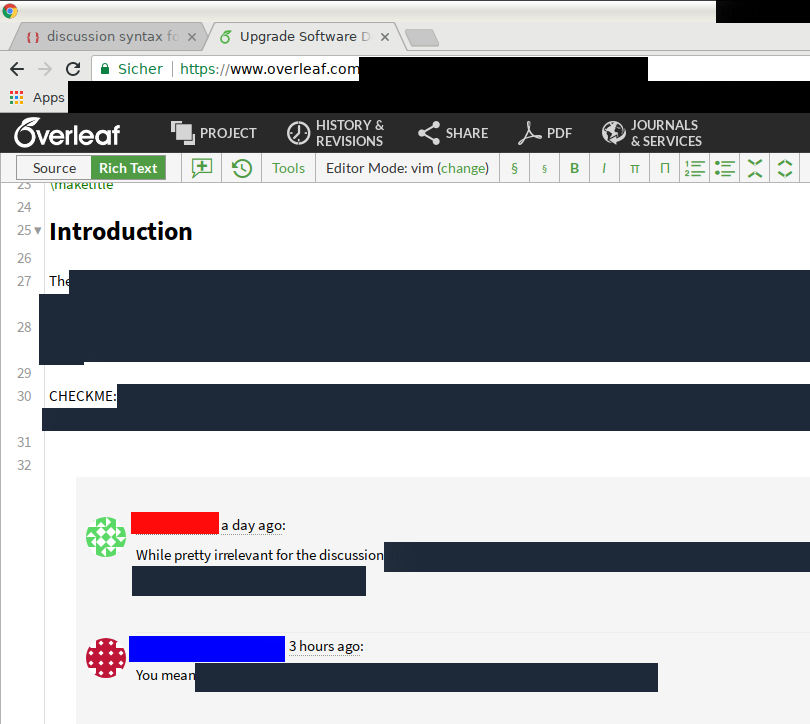
\includegraphics[height=.95\textheight]{./discuss_wysiwyg.png}

  \only<2>{
    \vspace{-.5\textheight}
    \begin{block}{Discussions kept in TeX comments}
      {\DejaSans ✓} discussions accessible through \texttt{git}

      {\DejaSans ✘} but \dots only really nice in the WYSIWYG view
    \end{block}
  }

\end{frame}

\section{problem}
\begin{frame}[t,fragile]
  \frametitle{discussions are error prone}
  \begin{lstlisting}[language=tex,gobble=2]
  % * <email@server.tld> 2018-02-05T14:56:52.585Z:
  %
  % I would phrase this similar ...
  %
  % ^ <other.email@server.tld> 2018-02-12T14:05:57.936Z:
  %
  % I agree, I just wanted to make it clear that I think this is a very hard problem.
  %
  % ^.
  \end{lstlisting}

  \begin{block}{only comments in the correct syntax get rendered}
    It happened to us multiple times that responses written in the source view in the browser were not seen byall users.
  \end{block}
  \only<2>{
    \vspace{-.6\textheight}
    \begin{alertblock}{That will happen again}
      \begin{itemize}
        \item if someone uses the page with default settings we can hardly blame them
        \item \dots maybe enforce WYSIWYG through non-technical means
      \end{itemize}
    \end{alertblock}
  }
  \only<3>{
    \vspace{-.6\textheight}
    \begin{exampleblock}{But maybe help where the issue is known}
      \begin{itemize}
        \item Getting the syntax right is easy for a computer
        \item[$\Rightarrow$] Let the computer do the job
      \end{itemize}
    \end{exampleblock}
  }

\end{frame}

\section{solution}
\begin{frame}
  \frametitle{I have something for you}
  \begin{block}{what's there}
    \begin{itemize}
      \item code on \myhref{https://github.com/pseyfert/overleaf-commenter}{https://github.com/pseyfert/overleaf-commenter}.
      \item mostly python for printing to the command line
      \item rudimentary vim plugin integration
        \begin{itemize}
          \item insert after cursor
          \item check if discussion already present (yes: reply, no: start)
        \end{itemize}
      \item code under AGPL, copyright with my employer
    \end{itemize}
  \end{block}
  \begin{exampleblock}{I'd be happy if this is of use for somebody}
    \begin{itemize}
      \item I'll be happy to merge a pull request with emacs integration
    \end{itemize}
  \end{exampleblock}
\end{frame}
\begin{frame}
  \frametitle{future developments}
  \begin{itemize}
    \item I tried overleaf v2 very early in the test phase
    \item direct \texttt{git} access is gone (only git\emph{hub} export/import)
      \begin{itemize}
        \item but overleaf says they're working on bringing it back
      \end{itemize}
    \item discussions not taking place in tex comments anymore
      \begin{itemize}
        \item[{\DejaSans ☹}] \texttt{overleaf-commenter} might become useless
        \item[{\DejaSans 😃}] no long term maintenance concerns
      \end{itemize}
  \end{itemize}

  
\includegraphics[width=.3\textwidth]{./QR2.png}
  \myhref{https://github.com/pseyfert/overleaf-commenter}{https://github.com/pseyfert/overleaf-commenter}.
\end{frame}

\appendix

\begin{frame}
  {\Huge{backup???}}

  {\sf{back up!}}
\end{frame}

\begin{frame}
  \frametitle{collaborative work on TeX documents is hard}

  Imagine you want to work with some colleagues on a LaTeX document
  \begin{block}{option 1: set up a git repo}
    \begin{itemize}
      \item \texttt{git clone/pull}, edit files, \texttt{make}, \texttt{git add}, \texttt{git commit}, \texttt{git push}, tell your colleagues to pull \dots for just fixing a typo???
      \item you don't see the same text when editing it during a skype call about 
        \newline (screen share requires good internet, only one can type)
    \end{itemize}
  \end{block}
  \begin{block}{option 2: work on the cloud in your browser}
    \begin{itemize}
      \item all your text editor configurations: gone
      \item bad hotel wifi: no work
    \end{itemize}
  \end{block}
\end{frame}



\end{document}
